\documentclass{article}

\usepackage{graphicx}
\usepackage{subfigure}

\usepackage{tikz}
\usetikzlibrary{positioning}

\begin{document}

\begin{figure}
  \centering
  \subfigure[Antes da operação]{
    \scalebox{0.7}{
      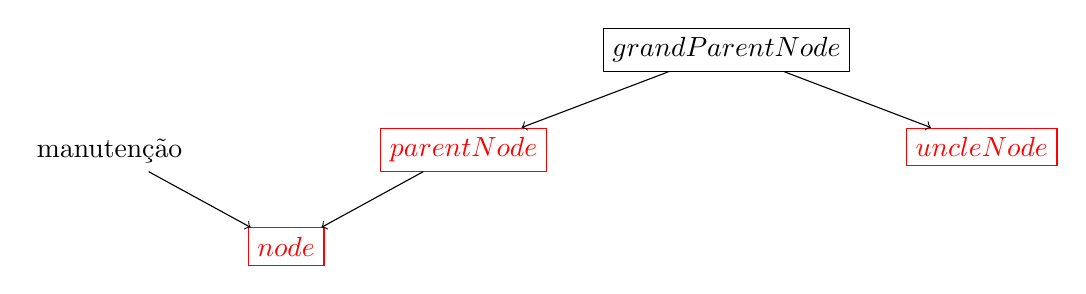
\begin{tikzpicture}
        \node[rectangle, draw, color = black] (gpNode) at (1, 1) {$grandParentNode$};
        \node[rectangle, draw, color = red] (pNode) [below left = 1cm of gpNode] {$parentNode$};
        \node[rectangle, draw, color = red] (uNode) [below right = 1cm of gpNode] {$uncleNode$};
        \node[rectangle, draw, color = red] (node) [below left = 1cm of pNode] {$node$};

        \node (m) [above left = 1cm of node] {manutenção};

        \draw (gpNode) edge[->] (pNode);
        \draw (gpNode) edge[->] (uNode);
        \draw (pNode) edge[->] (node);
        \draw (m) edge[->] (node);
      \end{tikzpicture}
    }
  }
  \subfigure[Depois da operação]{
    \scalebox{0.7}{
      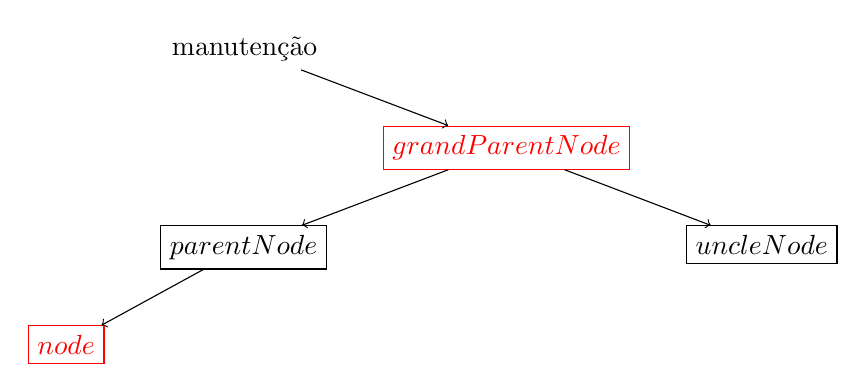
\begin{tikzpicture}
        \node[rectangle, draw, color = red] (gpNode) at (1, 1) {$grandParentNode$};
        \node[rectangle, draw, color = black] (pNode) [below left = 1cm of gpNode] {$parentNode$};
        \node[rectangle, draw, color = black] (uNode) [below right = 1cm of gpNode] {$uncleNode$};
        \node[rectangle, draw, color = red] (node) [below left = 1cm of pNode] {$node$};

        \node (m) [above left = 1cm of gpNode] {manutenção};

        \draw (gpNode) edge[->] (pNode);
        \draw (gpNode) edge[->] (uNode);
        \draw (pNode) edge[->] (node);
        \draw (m) edge[->] (gpNode);
      \end{tikzpicture}
    }
  }
  \caption{Ilustração do caso 1 da inserção.}
\end{figure}

\begin{figure}
  \centering
  \subfigure[Antes da operação]{
    \scalebox{0.7}{
      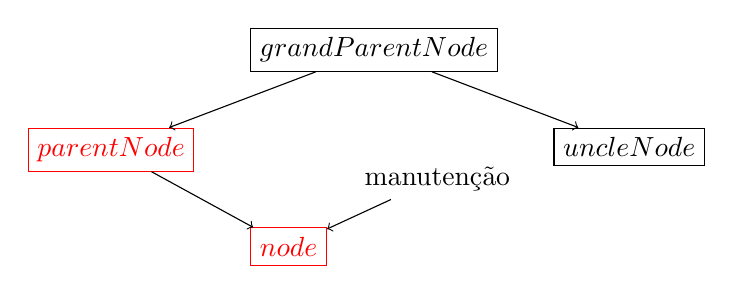
\begin{tikzpicture}
        \node[rectangle, draw, color = black] (gpNode) at (1, 1) {$grandParentNode$};
        \node[rectangle, draw, color = red] (pNode) [below left = 1cm of gpNode] {$parentNode$};
        \node[rectangle, draw, color = black] (uNode) [below right = 1cm of gpNode] {$uncleNode$};
        \node[rectangle, draw, color = red] (node) [below right = 1cm of pNode] {$node$};

        \node (m) [above right = 0.5cm of node] {manutenção};

        \draw (gpNode) edge[->] (pNode);
        \draw (gpNode) edge[->] (uNode);
        \draw (pNode) edge[->] (node);
        \draw (m) edge[->] (node);
      \end{tikzpicture}
    }
  }
  \subfigure[Depois da operação]{
    \scalebox{0.7}{
      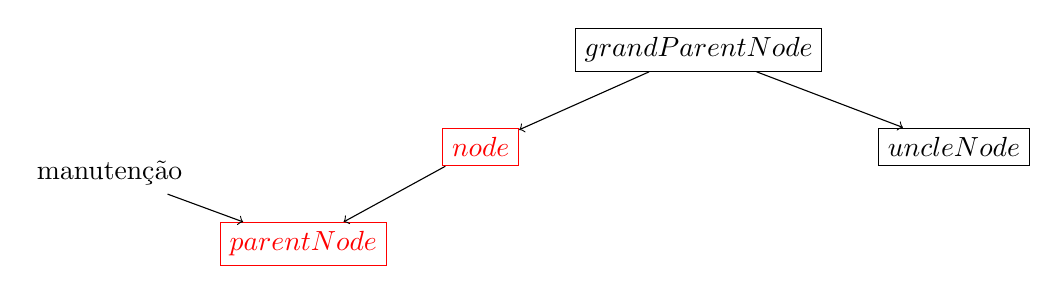
\begin{tikzpicture}
        \node[rectangle, draw, color = black] (gpNode) at (1, 1) {$grandParentNode$};
        \node[rectangle, draw, color = black] (uNode) [below right = 1cm of gpNode] {$uncleNode$};
        \node[rectangle, draw, color = red] (node) [below left = 1cm of gpNode] {$node$};
        \node[rectangle, draw, color = red] (pNode) [below left = 1cm of node] {$parentNode$};

        \node (m) [above left = 0.5cm of pNode] {manutenção};

        \draw (gpNode) edge[->] (node);
        \draw (gpNode) edge[->] (uNode);
        \draw (node) edge[->] (pNode);
        \draw (m) edge[->] (pNode);
      \end{tikzpicture}
    }
  }
  \caption{Ilustração do caso 2 da inserção.}
\end{figure}

\begin{figure}
  \centering
  \subfigure[Antes da operação]{
    \scalebox{0.7}{
      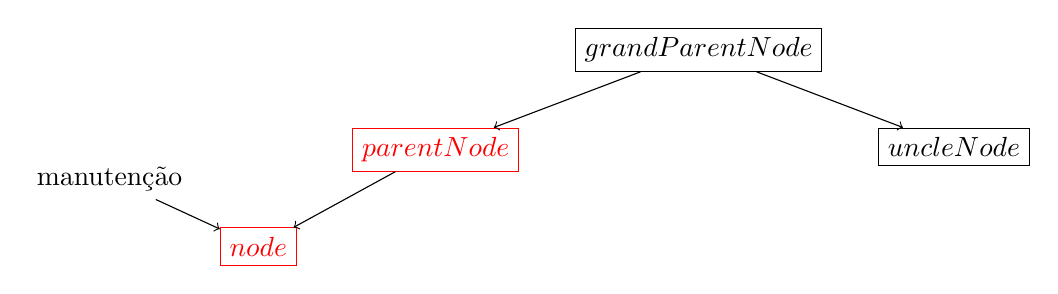
\begin{tikzpicture}
        \node[rectangle, draw, color = black] (gpNode) at (1, 1) {$grandParentNode$};
        \node[rectangle, draw, color = black] (uNode) [below right = 1cm of gpNode] {$uncleNode$};
        \node[rectangle, draw, color = red] (pNode) [below left = 1cm of gpNode] {$parentNode$};
        \node[rectangle, draw, color = red] (node) [below left = 1cm of pNode] {$node$};

        \node (m) [above left = 0.5cm of node] {manutenção};

        \draw (gpNode) edge[->] (pNode);
        \draw (gpNode) edge[->] (uNode);
        \draw (pNode) edge[->] (node);
        \draw (m) edge[->] (node);
      \end{tikzpicture}
    }
  }
  \subfigure[Depois da mudança de cores]{
    \scalebox{0.7}{
      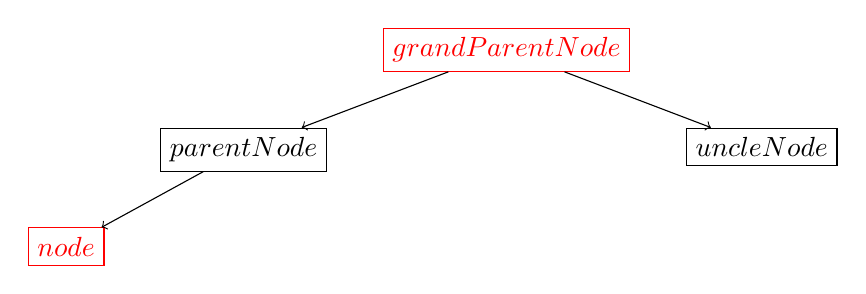
\begin{tikzpicture}
        \node[rectangle, draw, color = red] (gpNode) at (1, 1) {$grandParentNode$};
        \node[rectangle, draw, color = black] (uNode) [below right = 1cm of gpNode] {$uncleNode$};
        \node[rectangle, draw, color = black] (pNode) [below left = 1cm of gpNode] {$parentNode$};
        \node[rectangle, draw, color = red] (node) [below left = 1cm of pNode] {$node$};

        \draw (gpNode) edge[->] (pNode);
        \draw (gpNode) edge[->] (uNode);
        \draw (pNode) edge[->] (node);
      \end{tikzpicture}
    }
  }
  \subfigure[Depois da rotação]{
    \scalebox{0.7}{
      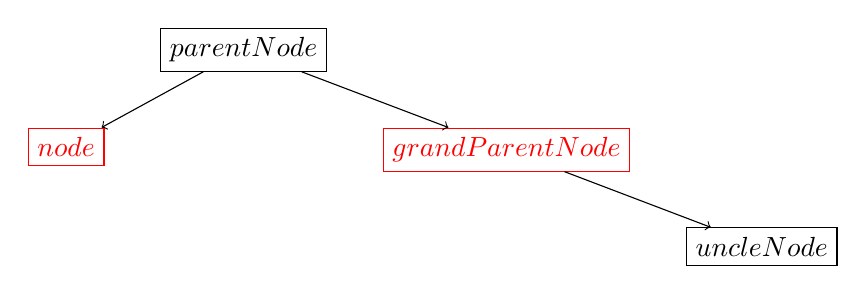
\begin{tikzpicture}
        \node[rectangle, draw, color = black] (pNode) at (1, 1) {$parentNode$};
        \node[rectangle, draw, color = red] (node) [below left = 1cm of pNode] {$node$};
        \node[rectangle, draw, color = red] (gpNode) [below right = 1cm of pNode] {$grandParentNode$};
        \node[rectangle, draw, color = black] (uNode) [below right = 1cm of gpNode] {$uncleNode$};

        \draw (pNode) edge[->] (node);
        \draw (gpNode) edge[->] (uNode);
        \draw (pNode) edge[->] (gpNode);
      \end{tikzpicture}
    }
  }
  \caption{Ilustração do caso 3 da inserção.}
\end{figure}

\end{document}

%%% Local Variables:
%%% mode: latex
%%% TeX-master: t
%%% End:
